\documentclass{beamer}
%[utf8,compress,handout]
\usetheme{JuanLesPins}

\usepackage[francais]{babel}
\usepackage[T1]{fontenc}
\usepackage[utf8]{inputenc}

\title{Modélisation et simulation de profils de comportement face à un incendie}
\author{Geoffrey DANET\\ supervisé par Carole ADAM\\équipe MAGMA}
\date{\today}

\expandafter\def\expandafter\insertshorttitle\expandafter{%
  \insertshorttitle\hfill%
}

\begin{document}

    \begin{frame}
        \titlepage
    \end{frame}

    \begin{frame}{Black Saturday}
            \begin{itemize}
                \item 7 février 2009,
                \item 173 morts et 414 blessés,
                \item \begin{math}\sim\end{math} 450 000 ha brûlés.
                \item Le comportement attendu est différent du comportement réel,
            \end{itemize}
        $\rightarrow$ Créer un jeu sérieux pour sensibiliser les décideurs au comportement réel de la population.
        \newline
        $\rightarrow$ Simulation le plus réaliste possible.
        \begin{figure}[h]
            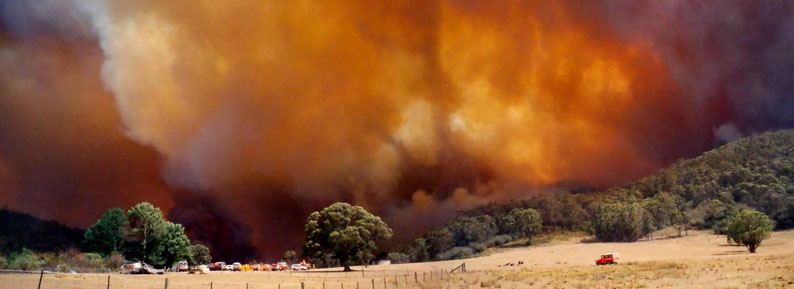
\includegraphics[scale=0.4]{canberra-2003-cropped.jpg}
        \end{figure}
    \end{frame}

    \begin{frame}{État de l'art}
        Les simulations existantes sont focalisées sur :
        \begin{itemize}
            \item Les comportements de foule pendant l'évacuation de bâtiments et de lieux publics,\cite{modeling2008}\cite{human2006}\cite{crowd2005}
            \begin{itemize}
                \item Évacuation,
                \item Navigation (recherche de chemin),
                \item Comportement basique et homogène.
            \end{itemize}
            \item Le comportement du feu, \cite{phoenix}
        \end{itemize}
        \begin{figure}[h]
            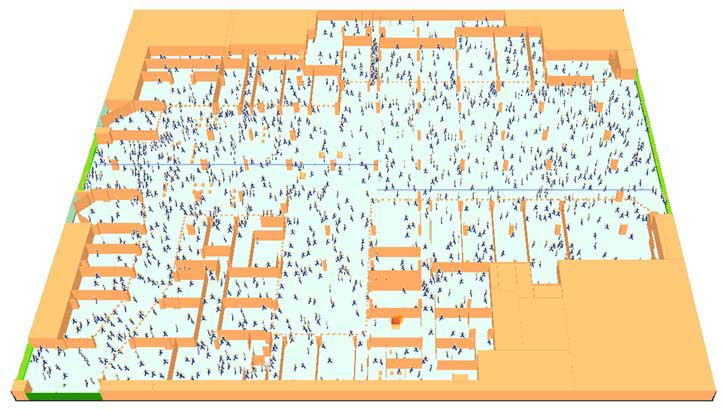
\includegraphics[scale=0.4]{eva.jpg}
        \end{figure}
    \end{frame}
    \begin{frame}{Proposition}
        \begin{itemize}
            \item Modéliser les différents comportements avec des agents BDI,
            \item Développer une simulation multi-agents (plateforme GAMA),
            \item Valider la simulation en la comparant avec les témoignages.
        \end{itemize}
        \begin{figure}[h]
            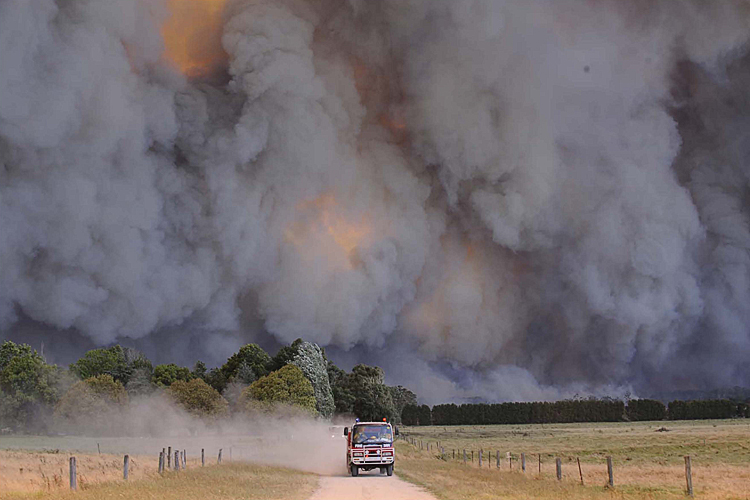
\includegraphics[scale=0.3]{PJ-1.jpg}
        \end{figure}
    \end{frame}

    \footnotesize
    \bibliographystyle{plain}
    \bibliography{biblio}

\end{document}
